\section{Owoce pod kruszonką}
\bigskip
\small
\begin{minipage}{0.45\textwidth}
    \noindent \textbf{Czas:} 60 minut \\
    \textbf{Poziom trudności:} łatwy
\end{minipage}
\begin{minipage}{0.45\textwidth}
    \noindent \textbf{Ilość sprzątania:} średnia\\
    \textbf{Wymagany mysi sprzęt:} -
\end{minipage}
\normalsize
\vspace{0.5cm}

\begin{multicols}{2}

\subsection*{Składniki}
\begin{itemize}
    \item 250 g ulubionych owoców zważonych bez pestek (śliwki, jabłka, truskawki, czereśnie, brzoskwinie, gruszki, itp.)
    \item 1 łyżka miodu
    \item 1 płaska łyżka mąki ziemniaczanej
    \item 0.3(3) szklanki mąki (może być pszenna, pełnoziarnista, owsiana)
    \item 2 łyżki płatków owsianych
    \item 2 łyżki cukru białego lub brązowego
    \item 0.25 kostki zimnego masła
    \item szczypta soli
\end{itemize}

\columnbreak

\begin{figure}[H]
    \centering
    \fbox{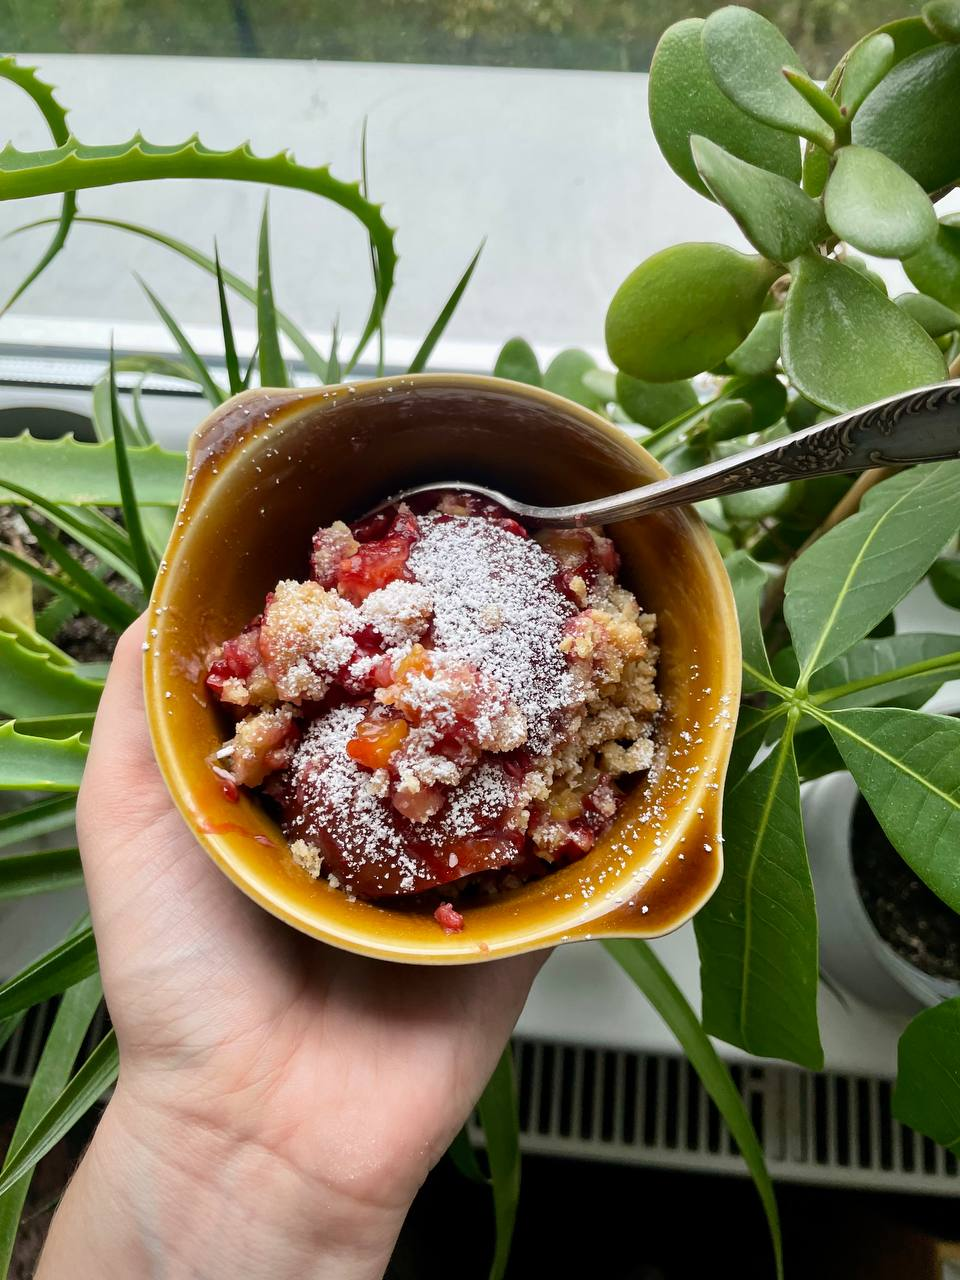
\includegraphics[width=0.35\textwidth]{images/kruszonka.jpg}}
\end{figure}
\end{multicols}

\vspace{0.5cm}

\subsection*{Instruktaż}
\begin{enumerate}
    \item Mąkę, płatki owsiane, szczyptę soli i cukier wymieszać dokładnie w misce i dodać masło pokrojone na małe kawałeczki. Rękami rozcierać masło razem z mąką, aż się połączą. Ciasto uformować w kulę, owinąć folią i wstawić do zamrażalnika na czas przygotowania owoców (10-15 minut).
    \item Piekarnik nagrzać do 180 stopni Celsjusza. Większe owoce jak brzoskwinie, śliwki, gruszki czy jabłka pokroić na kawałki przed włożeniem do naczynia żaroodpornego, polać miodem i posypać skrobią, po czym dokładnie wymieszać.
    \item Kruszonkę wyjąć z zamrażalnika i pokruszyć palcami lub zetrzeć na tarce i posypać nią owoce.
    \item Całość piec około 40 minut, do momentu aż kruszonka się zarumieni, a sok owocowy zacznie bulgotać.
\end{enumerate}

\vspace{0.5cm}

\small
\subsection*{Propozycja podania}
Z cukrem pudrem, z bitą śmietaną, z lodami, z jogurtem greckim.

\vspace{0.3cm}

\subsection*{Dodatkowe uwagi}
Nektarynki, brzoskwinie, czereśnie, borówki amerykańskie, maliny, truskawki, jeżyny, jagody, jabłka, gruszki, śliwki i morele – jeśli mrożone, należy piec 5 minut dłużej.

\newpage
